\documentclass[note=hide]{beamer} %für die Präsentation
%\documentclass[note=hide,handout]{beamer} %zum Drucken

\usepackage[utf8]{inputenc}
\usepackage{ngerman}
\usepackage[T1]{fontenc}

\usetheme{heidelberg}
%\usetheme{Malmoe}
%\usecolortheme{seahorse}
%\useoutertheme{smoothbars}

\usepackage{floatflt}
\usepackage{float}
\usepackage{graphicx}
\usepackage{hyperref}
\usepackage{color}

\usepackage{verbatim}
\usepackage{moreverb}
\usepackage{alltt}

\usepackage{comment}
\usepackage{booktabs}
\usepackage{rotating}
\usepackage{fixltx2e}
\usepackage{tikz}
\usepackage{multirow}
\usepackage{gantt}


\usetikzlibrary{positioning,shadows,shapes,arrows}
% color definitions
\definecolor{dunkelrot}{RGB}{139, 0, 0} 
\definecolor{dunkelgruen}{RGB}{0,100,0}
\definecolor{mildesgruen}{RGB}{154,255,154}
\definecolor{orange}{RGB}{255,140,105}
\definecolor{mildesorange}{RGB}{255,140,105}
\definecolor{dunklesgruen}{RGB}{0, 139, 69}
\definecolor{cyan}{RGB}{24, 116, 205}
%\usepackage{colortbl}
%\usepackage{tabular}


\definecolor{dkgreen}{rgb}{0,0.6,0}
\definecolor{gray}{rgb}{0.5,0.5,0.5}
\definecolor{mauve}{rgb}{0.58,0,0.82}

%Damit wir Quellcode nutzen können.

\usepackage{listingsutf8}
\lstset{inputencoding=latin1}
\lstset{literate=%
	{Ö}{{\"O}}1
	{Ä}{{\"A}}1
	{Ü}{{\"U}}1
	{ß}{{\ss}}2
	{ü}{{\"u}}1
	{ä}{{\"a}}1
	{ö}{{\"o}}1
}
\lstset{numbers=left,
	numberstyle=\tiny,
	numbersep=5pt,
	breaklines=true,
	showstringspaces=false,
	frame=l ,
	xleftmargin=15pt,
	xrightmargin=15pt,
	basicstyle=\ttfamily\tiny,
	stepnumber=1,
	keywordstyle=\color{blue},          % keyword style
	commentstyle=\color{dkgreen},       % comment style
	stringstyle=\color{mauve}         % string literal style
}
%Sprache Festelegen
\lstset{language=Python}
%Beispiele
%-> \begin{lstlisting}[language=JAVA,firstnumber=27] ... \end{lstlisting}
%-> \lstinline[language=JAVA]{...}
%-> for beamer, embed it in a fragile frame!: \begin{frame}[fragile]{Beispiel} ... \end{frame}

\title[<SPaMMT>]{Semantic Parsing as \\ Monolingual Machine Translation} %Einen Kürzel für das Referatsthema angeben (erscheint im zweiten Feld der Fußzeile).
\subtitle{Software Projekt Sommersemester 2016} %Titel des Referats angeben
\author[SNMaxYMarO]{Stoyan Dimitrov -- Nadja Heinzen \\ Maximilian Lapp\'{e} -- Yoalli Rezepka Garc\'{i}a\\ Marina Speranskaya -- Ozan Yilmaz} %Namen bitte in alphabetischer Reihenfolge angeben. Namenkürzel zusätzlich angeben (erscheint im dritten Feld der Fußzeile).
\institute[]{Ruprecht-Karls-Universität Heidelberg 
	\\ Institut für Computerlinguistik
	\\ Betreuer: Prof. Dr. Stefan Riezler
	\vspace{5pt}
	\\ Folien beinhalten Materialien von Carolin Haas	
}
	
\date{31.05.2016} %oder ein vorgegebenes Datum; soll nicht zu lang sein, weil das Datum auch in das linke Feld der Fußzeile passen soll.

\begin{document}

\begin{frame}[plain]
	\titlepage
\end{frame}
\begin{frame}
	\tableofcontents
\end{frame}

\section{Themenvorstellung}
\begin{frame}{Themenvorstellung}
	\begin{minipage}{0.73\textwidth}
		\begin{itemize}
		\item \textbf{Thema}: Semantic Parsing as Monolingual \\ \hspace{42pt}Machine Translation
		\begin{itemize}
			\item\textbf{Hauptziel}
		\begin{itemize}
			\item Baseline von Carolin Haas nachbauen und verbessern
			\item NLMaps erweitern
			\item SMT-Teil durch Neuronale Netze ersetzen 
		\end{itemize} 			
		\end{itemize}
		\end{itemize}
	\end{minipage}
	\hfill
	\begin{minipage}{0.25\textwidth}
	\begin{figure}[b]
				\vspace{115pt}		
				\includegraphics[width= 3.5 cm]{E:/LaTex/Dateien/Präsentation-EML/Gruppenarbeit.jpg}		
	\end{figure}
	\end{minipage}
\end{frame}

\begin{frame}{NLMaps Korpus}
	\begin{itemize}
		\item von Carolin Haas zusammengestellt
		\item besteht aus 2380 Fragen über geografische Fakten
		\item Fragen können mit Hilfe der OpenStreetMap Datenbank beantwortet werden
		\item Jede Frage besitzt eine korrespondierende MRL (Machine Readable Language) Formel, welche auf Overpass basiert
	\end{itemize}
	\textbf{Beispiel:}\\
	``Which hotels in Paris have wheelchair access?''\\
	-> query(area(keyval('name','Paris')),\\nwr(keyval('tourism','hotel'),keyval('wheelchair','yes')),findkey('name'))
\end{frame}

\begin{frame}{NLMaps Interface}
	\begin{minipage}{0.64\textwidth}
		\flushleft
		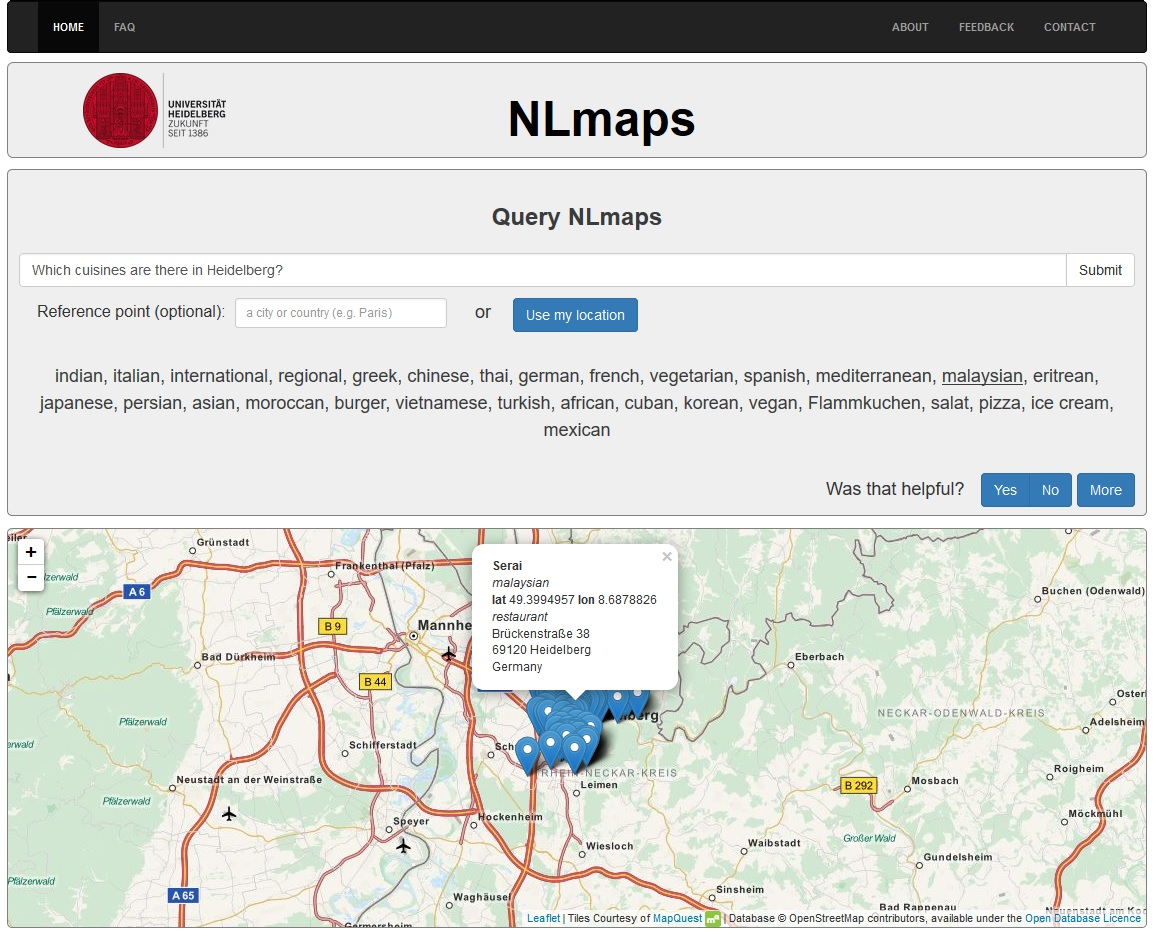
\includegraphics[width=\textwidth]{interface.jpg}
	\end{minipage}
	\hfill
	\begin{minipage}{0.34\textwidth}
		\flushright
	\begin{itemize}
		\item von Carolin Haas erstellt
		\item Benutzer können eine natürlichsprachliche Anfrage stellen, welche von dem System verarbeitet und schließlich beantwortet wird
	\end{itemize}
\end{minipage}
\end{frame}

\begin{frame}{Ablauf}
	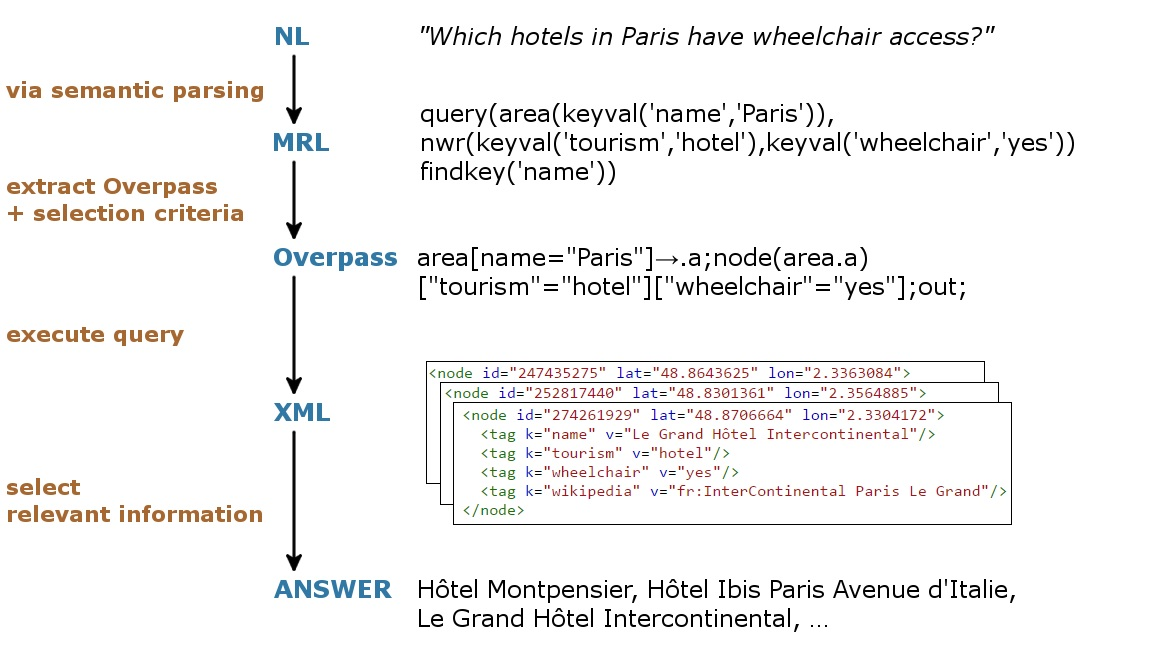
\includegraphics[width=\textwidth]{pipeline.jpg}
\end{frame}

\begin{frame}{OpenStreetMap}
	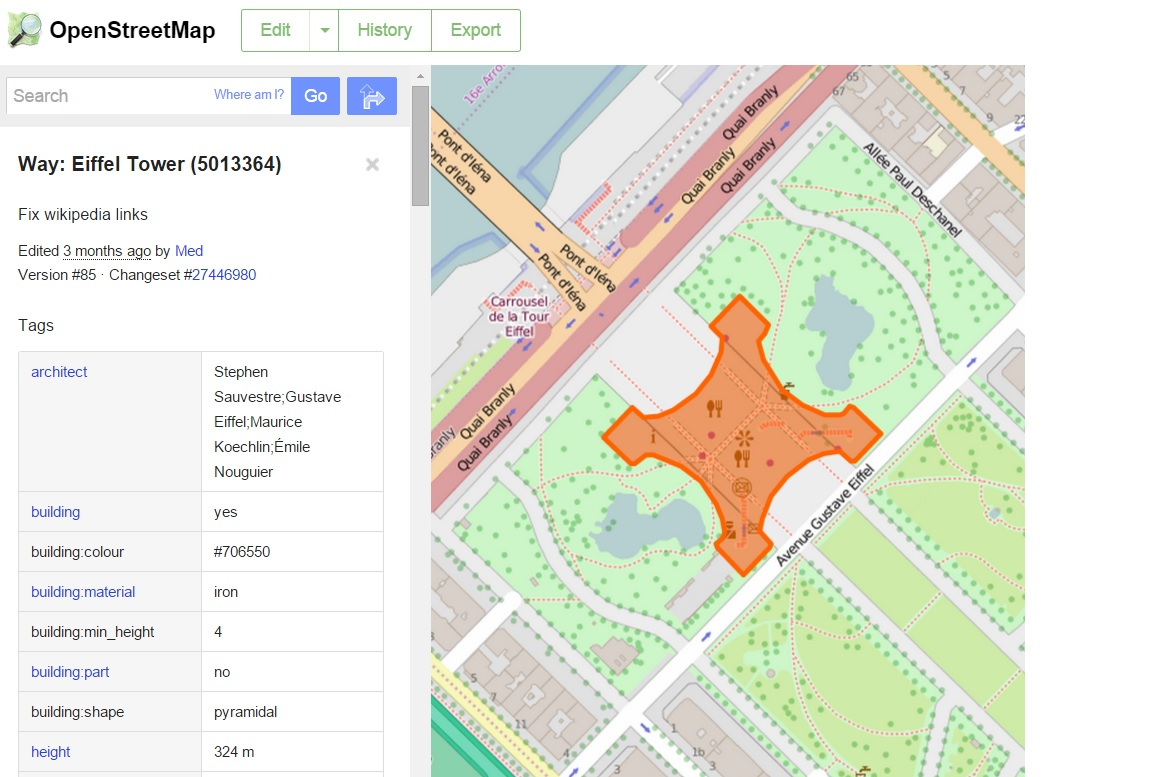
\includegraphics[width=\textwidth]{openstreetmap.jpg}
\end{frame}

\begin{frame}{Overpass}
	\begin{minipage}{0.64\textwidth}
		\flushleft
		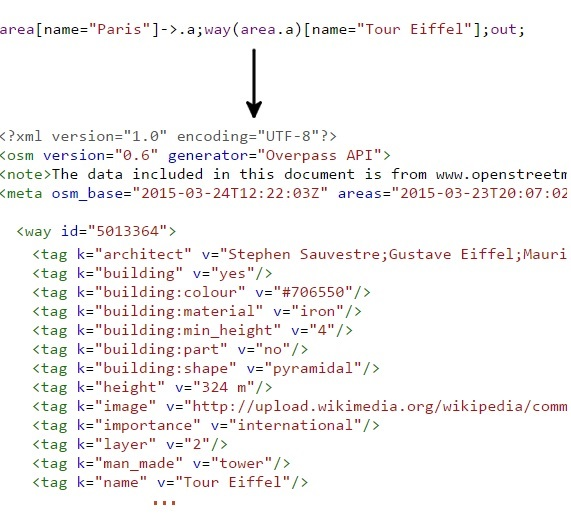
\includegraphics[width=\textwidth]{overpass.jpg}
	\end{minipage}
	\hfill
	\begin{minipage}{0.34\textwidth}
		\flushright
		\begin{itemize}
			\item 
		\end{itemize}
	\end{minipage}
\end{frame}
\section{Projektverlauf}
\begin{frame}{Projektverlauf}
	\begin{figure}[H]
		\centering{
			\resizebox{0.5\textwidth}{!}{	\tikzstyle{decision} = [diamond, draw, fill=blue!20, 
	text width=4.5em, text badly centered, node distance=3cm, inner sep=0pt]
	\tikzstyle{block} = [rectangle, draw, fill=cyan!50, 
	text width=8em, text centered, rounded corners, minimum height=4em]
	\tikzstyle{line} = [draw, -latex']
	\tikzstyle{cloud} = [draw, ellipse,fill=red!20, node distance=3cm,
	minimum height=2em]

		\begin{tikzpicture}[node distance = 2cm, auto]
		% Place nodes
		
		\node [block] at (6 ,9) (daten){Daten (NLMaps Anfrage - Overpass)};
		\node [block] at (6 ,6.5) (linear){Linearisierung der MRL};
		\node [block] at (1 ,4) (neural){Neural Networks};
		\node [block] at (6 ,4) (language){Language Model};
		\node [block] at (11 ,4) (align){Alignment Model};
		\node [block] at (8.5, 1.5) (decoder){Decoder};
		\node [block] at (6, -1) (delinear){Delinearisierung};
		\node [block] at (6 ,-3.5) (cfg){CFG Kontrolle};
		\node [block] at (6 ,-6) (overpass){\"Uberf\"uhrung in Overpass};
		\node [block] at (6 ,-8.5) (schnitt){Schnittstelle Carolin Haas};	
		% Draw edges
		\draw[->, very thick] (6,8) --  node[label= right:MRL in Klammerstruktur] {} (6,7.3);
		\draw[->, very thick] (4.4,8.1) --  node[] {} (2.5,4.8);
		\draw[->, very thick] (7.5,8.1) --  node[] {} (9.5,4.8);
		\draw[->, very thick] (6,5.6) --  node[] {} (6,5);
		\draw[->, very thick] (6,5.6) --  node[] {} (2.7,4.8);
		\draw[->, very thick] (6,5.6) --  node[] {} (9.3,4.8);
		\draw[->, very thick] (6,3.2) --  node {} (8.4,2.4);
		\draw[->, very thick] (11,3.2) --  node {} (8.6,2.4);
		\draw[->, very thick] (1,3.2) --  node {} (4.4,-0.2);
		\draw[->, very thick] (8.5,0.7) --  node {} (7.7,-0.2);	
		\draw[->, very thick] (6,-1.8) --  node[label=right:MRL in Klammerstruktur] {} (6,-2.7);	
		\draw[->, very thick] (6,-4.3) --  node[label= right: konformer MRL-Ausdruck] {} (6,-5.2);
		\draw[->, very thick] (6,-6.8) --  node[label=right: Overpass Abfrage] {} (6,-7.6);
		
		\end{tikzpicture}}}		
	\end{figure}
\end{frame}
\section{Organisatorisches}
\begin{frame}{Arbeitsverteilung}
	\begin{table}[H]
		\normalsize		
		\begin{tabular}{|c|c|c|}
			\hline
			\textbf{Person} & \textbf{Aufgabe}  & \textbf{Programm} \\
			\hline
			Ozan & MRL linearisieren & eigenes Programm \\
			\hline
			Yoalli & CFG überprüfen & evtl. vorhandenes Programm \\ 
			\hline
			Nadja & Alignment & nltk.align \\
			\hline
			Ozan & Decoder & nltk.translate \\
			\hline
			Marina & Language Model & nltk.model.ngram \\
			\hline
			Max, Stoyan & Neural Networks & TensorFlow Seq.-to-Seq.\\
			\hline
			alle & Korpuserweiterung & Interface NLMaps\\
			\hline			
		\end{tabular}		
	\end{table}
\end{frame}	

\begin{frame}{Zeitplan}
	\begin{figure}[H]
		\centering{
			\resizebox{0.9\textwidth}{!}{\begin{gantt}{13}{13}
	\begin{ganttitle}
		\numtitle{1}{1}{13}{1}
	\end{ganttitle}
	\ganttbar{theor. Grundlagen}{0}{3}
	\ganttbar{MRL linearisieren}{4}{1}
	\ganttbar{CFG {\"u}berpr{\"u}fen}{4}{1}
	\ganttbar{Alignment}{5}{4}
	\ganttbar{Decoder}{6}{4}
	\ganttbar{Language Model}{7}{4}
	\ganttmilestone[color=cyan]{Abgabe Forschungsplan}{3}
	\ganttmilestone[color=cyan]{Projektspez.-vortrag}{4}
	\ganttbar{Neural Networks}{4}{7}
	\ganttbar[color=cyan]{Korpuserweiterung}{4}{7}
	\ganttmilestone[color=cyan]{Demo}{12}
	\ganttmilestone[color=cyan]{Abgabe}{13}	
\end{gantt}}}		
	\end{figure}	
\end{frame}

\begin{frame}{Quellen}
	
	Jacob Andreas, Andreas Vlachos und Stephen Clark. “Semantic Parsing as
	Machine Translation.” In: ACL (2). 2013, S. 47–52. \\ \vspace{5pt}
	Kyunghyun Cho u. a. “Learning Phrase Representations using RNN Encoder-
	Decoder for Statistical Machine Translation”. In: CoRR abs/1406.1078 (2014).
	url: http://arxiv.org/abs/1406.1078. \\ \vspace{5pt}
	Carolin Haas und Stefan Riezler. “A Corpus and Semantic Parser for Multilingual
	Natural Language Querying of OpenStreetMap”. In: ().\\ \vspace{5pt}
	\url{https://t1.ftcdn.net/jpg/00/69/46/42/240_F_69464288_SyWbOA5zDkntO6pTCAtapSDlkzK4qsm9.jpg}
\end{frame}

\end{document}
